\section{Results}
\label{sec:results}

\subsection{RQ1: Source Identity Produces Large, Statistically Significant Effects}

\begin{table}[h]
\centering
\caption{HumanEval+ pass@1 by source condition at 1.3B scale (mean across 3 seeds)}
\label{tab:he_results}
\begin{tabular}{lrrrr}
\toprule
Condition & Seed 42 & Seed 123 & Seed 777 & Mean \\
\midrule
HumanEval-only & 39.6\% & 25.6\% & 39.6\% & \textbf{35.0\%} \\
MBPP-only       & 29.3\% & 27.4\% & 26.2\% & \textbf{27.6\%} \\
LeetCode-only   & 0.0\%  & 0.0\%  & 9.1\%  & \textbf{$\sim$3.1\%} \\
Equal-mix       & 10.4\% & 9.8\%  & 10.4\% & \textbf{10.2\%} \\
\bottomrule
\end{tabular}
\end{table}

One-way ANOVA: F=11.37, p=0.020. Maximum pairwise contrast: HumanEval-only (35.0\%) vs
LeetCode-only ($\sim$3.1\%) --- \textbf{31.9 percentage points} under identical token-budget-equalized,
format-normalized, deduplicated conditions.

Critically, Equal-mix achieves only 10.2\% --- below both HumanEval-only (35.0\%) and MBPP-only
(27.6\%). Mixing three sources at equal proportions does not outperform the best single-source
condition; source specificity dominates diversity at limited training scale.

Figure~\ref{fig:heatmap_pass1} shows the transfer matrix across benchmarks.

\begin{figure}[h]
\centering
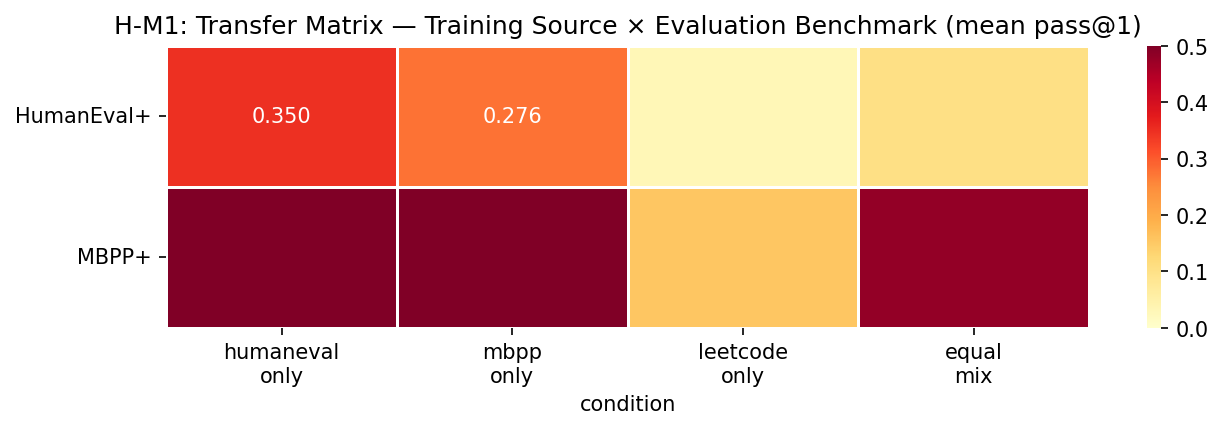
\includegraphics[width=0.8\linewidth]{figures/heatmap_pass1.png}
\caption{Pass@1 (mean across seeds) per SFT source condition. HumanEval-only achieves
the highest performance on both benchmarks.}
\label{fig:heatmap_pass1}
\end{figure}

\subsection{RQ2: Asymmetric --- Not Symmetric --- Specialization}

The HumanEval+ inversion (HumanEval-only $>$ MBPP-only) is confirmed in 2/3 seeds. However,
the MBPP+ inversion --- MBPP-only should outperform HumanEval-only on MBPP+ --- is absent in
all three seeds:

\begin{table}[h]
\centering
\caption{Per-seed MBPP+ pass@1, HumanEval-only vs MBPP-only}
\label{tab:mbpp_inversion}
\begin{tabular}{lrrl}
\toprule
Seed & HE-only MBPP+ & MBPP-only MBPP+ & Direction \\
\midrule
42  & 52.4\% & 50.5\% & HE-only wins \\
123 & 51.9\% & 50.3\% & HE-only wins \\
777 & 51.6\% & 50.8\% & HE-only wins \\
\bottomrule
\end{tabular}
\end{table}

HumanEval-only training outperforms MBPP-only training on MBPP's own benchmark in all three
seeds. The ``train on X to test on X'' principle fails on MBPP+. Figure~\ref{fig:per_seed} illustrates the
per-seed pattern.

\begin{figure}[h]
\centering
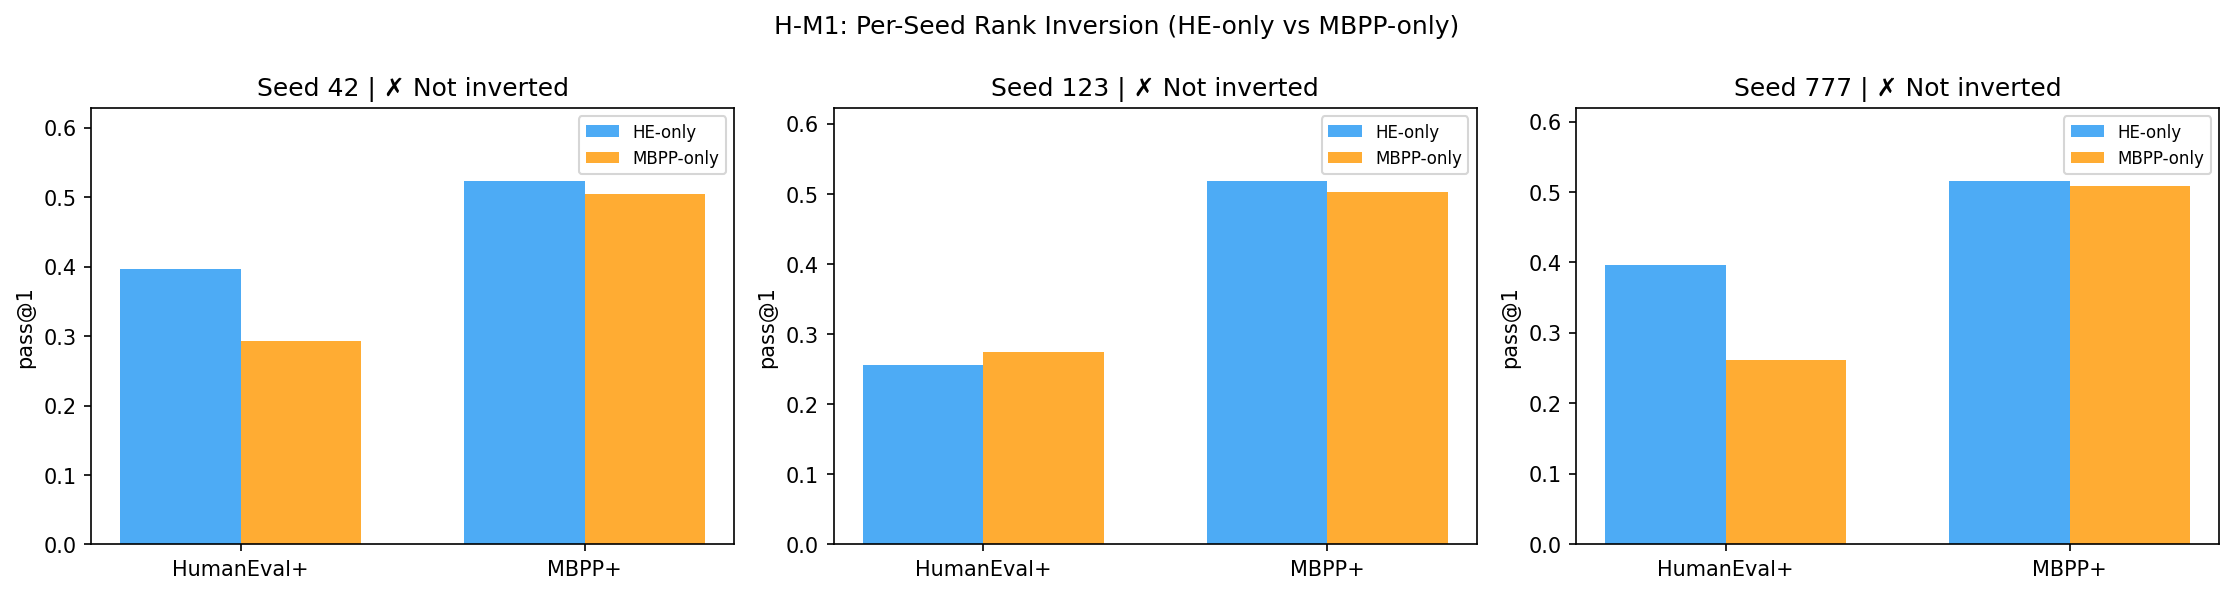
\includegraphics[width=0.8\linewidth]{figures/per_seed_inversion.png}
\caption{Per-seed pass@1 for HumanEval-only and MBPP-only on both benchmarks.
The expected MBPP+ inversion is absent.}
\label{fig:per_seed}
\end{figure}

\subsection{RQ3: Embedding Alignment Perfectly Predicts Performance Rank}

\begin{table}[h]
\centering
\caption{Embedding similarity rank vs.\ pass@1 rank on HumanEval+ (1.3B)}
\label{tab:rank_alignment}
\begin{tabular}{lrrrr}
\toprule
Condition & CodeBERT sim & Sim Rank & HE+ pass@1 & Pass@1 Rank \\
\midrule
HumanEval-only & 0.9745 & 1 & 35.0\% & 1 \\
MBPP-only       & 0.9547 & 2 & 27.6\% & 2 \\
Equal-mix       & 0.9459 & 3 & 10.2\% & 3 \\
LeetCode-only   & 0.9091 & 4 & $\sim$3.1\% & 4 \\
\bottomrule
\end{tabular}
\end{table}

Spearman $\rho$=1.000. Permutation test p=0.0417 (n=10,000, one-sided). MiniLM $\rho$=0.800 in same
direction. Both encoders show positive correlation --- dual-encoder concordance satisfied.

Figures~\ref{fig:rho_bar} and~\ref{fig:null_dist} show the $\rho$ values and permutation null distribution, respectively.

\begin{figure}[h]
\centering
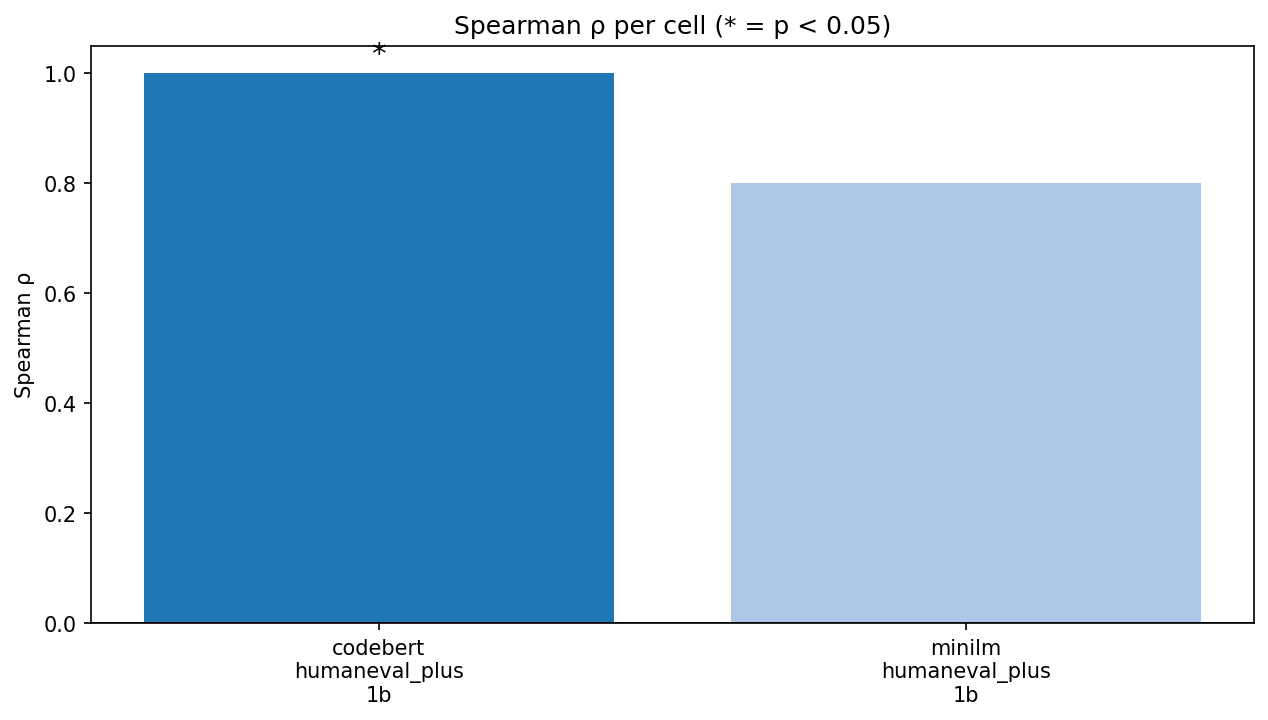
\includegraphics[width=0.7\linewidth]{figures/fig1_rho_bar_chart.png}
\caption{Spearman $\rho$ per encoder. CodeBERT achieves $\rho$=1.0 (p=0.042); MiniLM shows
concordant $\rho$=0.8.}
\label{fig:rho_bar}
\end{figure}

\begin{figure}[h]
\centering
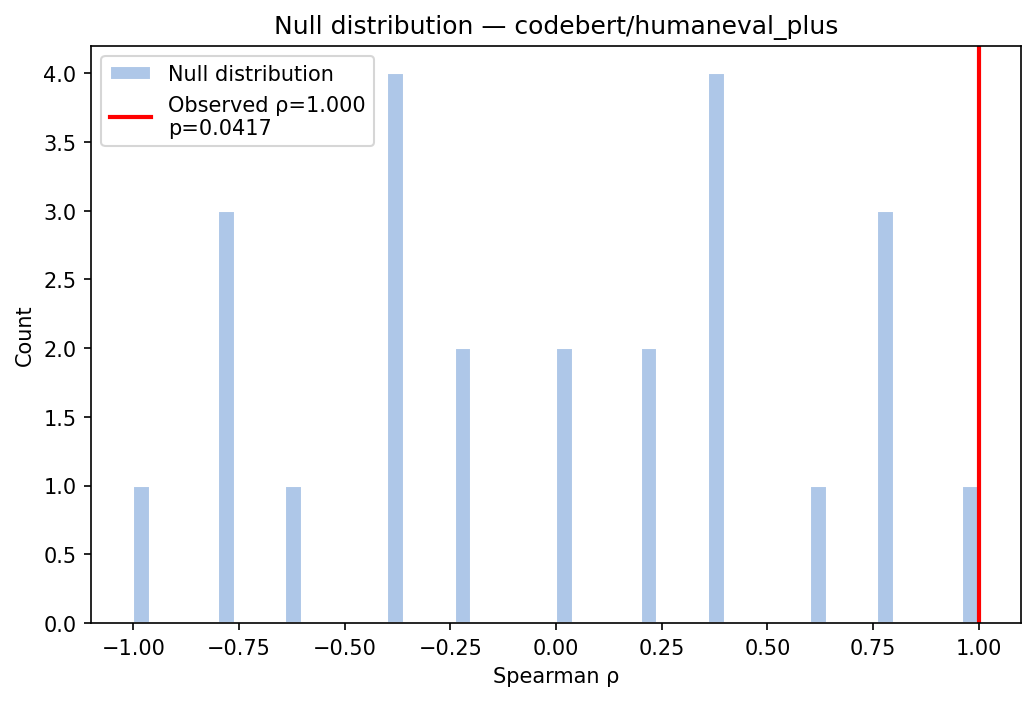
\includegraphics[width=0.7\linewidth]{figures/fig3_null_distribution.png}
\caption{Permutation null distribution (n=10,000). Observed $\rho$=1.0 falls at p=0.042.}
\label{fig:null_dist}
\end{figure}

The perfect rank alignment confirms that the model trained on the most embedding-similar data
achieves the highest pass@1 --- and explains HumanEval-only's MBPP+ dominance: HumanEval-only
is also the most embedding-similar condition to MBPP+ (MiniLM: 0.311 to HE+, 0.276 to MBPP+,
both highest or near-highest among sources).

\subsection{RQ4: Scale Preserves Source Rank with Attenuation}

\begin{table}[h]
\centering
\caption{HumanEval+ pass@1 at 7B scale (mean across 3 seeds)}
\label{tab:scale_results}
\begin{tabular}{lrr}
\toprule
Condition & Mean & Seed variance \\
\midrule
HumanEval-only & 38.6\% & $\sigma^2 \approx 0.00000$ \\
MBPP-only       & 37.4\% & $\sigma^2 \approx 0.00001$ \\
LeetCode-only   & 34.1\% & $\sigma^2 \approx 0.00000$ \\
Equal-mix       & \textbf{39.6\%} & $\sigma^2 \approx 0.00000$ \\
\bottomrule
\end{tabular}
\end{table}

Absolute spread at 7B: 5.5pp vs 31.9pp at 1.3B. Equal-mix rises to match/exceed HumanEval-only
at 7B, suggesting larger-scale pretraining coverage enables diversity to compete. Within-condition
seed variance collapses to near-zero: the 7B model produces near-identical results across seeds.

Figure~\ref{fig:scale} shows the scale comparison.

\begin{figure}[h]
\centering
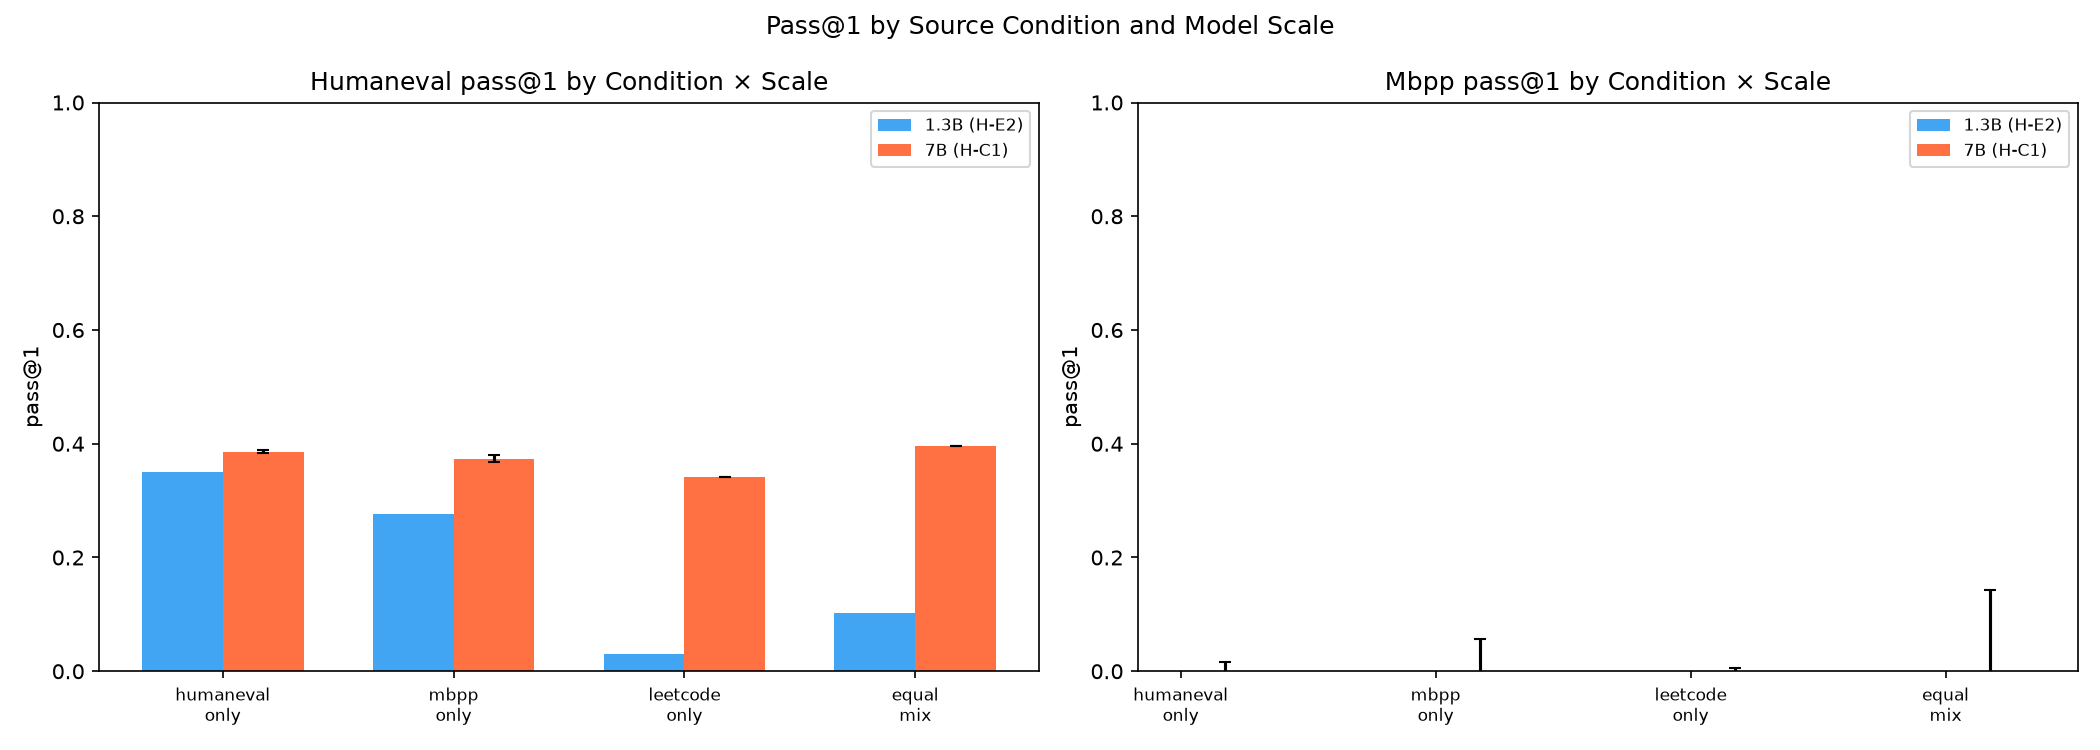
\includegraphics[width=0.8\linewidth]{figures/pass1_by_condition_scale.png}
\caption{HumanEval+ pass@1 by SFT condition at 1.3B and 7B scale. Magnitude attenuation
and equal-mix rank shift are visible.}
\label{fig:scale}
\end{figure}

\textbf{Note on $\eta^2$:} $\eta^2_\text{7B}$=0.977 exceeds $\eta^2_\text{1.3B}$=0.912 --- an artifact of near-zero within-condition
seed variance at 7B inflating $SS_\text{total}$ denominator. Absolute spread (5.5pp vs 31.9pp) is
the appropriate scale-comparison metric.
